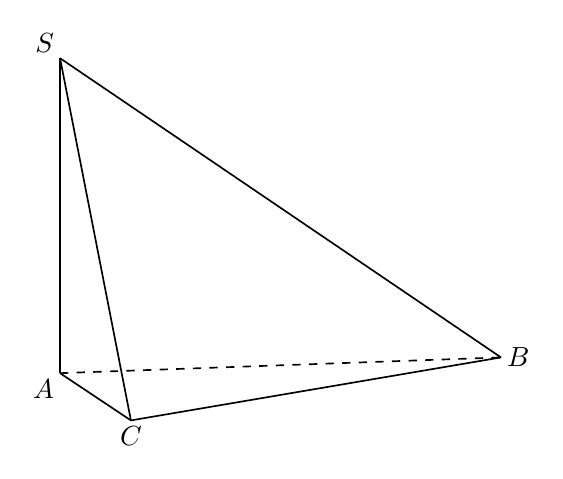
\begin{tikzpicture}[x=1cm,y=1cm,font=\normalsize,
  geometry edge/.style={solid,line width=.6pt},
  geometry label/.style={font=\normalsize,inner sep=2pt}]
\coordinate (S) at (0.6,5.2);
\coordinate (A) at (0.6,1.2);
\coordinate (C) at (1.5,0.6);
\coordinate (B) at (6.2,1.4);
\draw[geometry edge] (S)--(A);
\draw[geometry edge] (S)--(C);
\draw[geometry edge] (S)--(B);
\draw[geometry edge] (A)--(C)--(B);
\draw[geometry edge,dashed] (A)--(B);
\node[geometry label,above left] at (S) {$S$};
\node[geometry label,below left] at (A) {$A$};
\node[geometry label,below] at (C) {$C$};
\node[geometry label,right] at (B) {$B$};
\end{tikzpicture}
